\documentclass[en,11pt]{latex/elegantbookr}

\usepackage{natbib}
\bibliographystyle{plainnat}

\hypersetup{
  pdfcreator={LaTeX via pandoc}}


\usepackage{longtable,booktabs}



\setlength{\emergencystretch}{3em}  % prevent overfull lines
\providecommand{\tightlist}{%
  \setlength{\itemsep}{0pt}\setlength{\parskip}{0pt}}

\setcounter{secnumdepth}{5}

%%% Use protect on footnotes to avoid problems with footnotes in titles
\let\rmarkdownfootnote\footnote%
\def\footnote{\protect\rmarkdownfootnote}

  \title{Algebra and Geometry of Elementary Functions}


  \author{Fei Ye}

  \date{2020-01-27}

% logo 图案
% 封面图片
% 版本号
  \version{0.01}
% 机构名
% 引用格言
% 导言区 preamble
\usepackage{framed,color}
\definecolor{shadecolor}{RGB}{248,248,248}


%%%%%%%%%%%%%%%%%%%%%%%%% Adjust words spacing %%%%%%%%%%%%%%%%%%
\usepackage[protrusion=true,expansion=true]{microtype}
%%%%%%%%%%%%%%%%%%%%%%%%%%%%%%%%%%%%%%%%%%%%%%%%%%%%%%%%%%%%%%%%%

%%%%%%%%%%%%%%%%%%% Packages for Math %%%%%%%%%%%%%%%%%%%%%%%%%%
\usepackage{mathtools}
% \usepackage{breqn}
%%%%%%%%%%%%%%%%%%%%%%%%%%%%%%%%%%%%%%%%%%%%%%%%%%%%%%%%%%%%

%%%%%%%%%%%%%%%%%%%%%%%%%% Font Encoding Packages %%%%%%%%%%%%%%%%%%%%%%%
% \usepackage[utf8]{inputenc}

% \usepackage[T1]{fontenc}  % use this if European fonts (ec) package is installed
%%%%%%%%%%%%%%%%%%%%%%%%%%%%%%%%%%%%%%%%%%%%%%%%%%%%%%%%%%%%%%%%%%%%%%%%%%%%%%

%%%%%%%%%%%%%%%%%%%%%%%%%%%%%% Font Packages %%%%%%%%%%%%%%%%%%%%%%%%%%%%%%%
% \usepackage{libertine}  %%%%%The Linux Libertine font family
% \usepackage[libertine]{newtxmath}

% \usepackage[expert,altbullet,vargreek,noamssymbols]{lucidabr}
% \usepackage[expert,vargreek,noamssymbols]{lucbmath}


% \usepackage{charter}    %%%%%%Good for screen display
% \usepackage[charter]{mathdesign}
%%%%%%%%%%%%%%%%%%%%%%%%%%%%%%%%%%%%%%%%%%%%%%%%%%%%%%%%%%%%%%%%%%%%%%%%%%%%%%%%%%%%%%%%%

\hypersetup{
	linktoc=all
}

\usepackage{color}
% \usepackage[table]{xcolor}

\definecolor{greenbean}{RGB}{144,237,204}
%\pagecolor{greenbean}
\def\gray{\color{gray}}
\def\black{\color{black}}
\def\blue{\color{blue}}
\def\red{\color{red}}
\def\green{\color{green}}
\def\yellow{\color{yellow}}
\def\cyan{\color{cyan}}
\def\brown{\color{brown}}
\def\purple{\color{purple}}
\def\olive{\color{olive}}
\def\lime{\color{lime}}
\def\darkgray{\color{darkgray}}

%%%%%%%%%%%%%%%% Include Graphs %%%%%%%%%%%%%%%%%%%%%%
\usepackage{float}
\textfloatsep=0pt
\dblfloatsep=0pt
%%%%%%%%%%%%%%%%%%%%%%%%%%%%%%%%%%%%%%%%%%%%%%%%%%%%%%

%%%%%%%%%%%%%% Spacing for Baseline and Parskip  %%%%%%%%%%%%%%
\renewcommand{\baselinestretch}{1.1}
%%%%%%%%%%%%%%%%%%%%%%%%%%%%%%%%%%%%%%%%%%%%%%%%%%%%%%%%%%%%%%%

%%%%%% Packages for Fine Tune Content %%%%%%%%%%%
\usepackage[english]{babel}
\usepackage{indentfirst,bm}
%%%%%%%%%%%%%%%%%%%%%%%%%%%%%%%%%%%%%%%%%%%%%%%%%

%%%%%%%%%%%%%%%%%%%%%%%%%%%%%%%%%%%%%%%%%%%%%%%%%
% \usepackage{hhline}
%%%%%%%%%%%%%%%%%%%%%%%%%%%%%%%%%%%%%%%%%%%%%%%%%%%

%%%%%%%%%%%%%%%%%%%%%%%%%%%%%%%%%%%%%%%%%%%%%%%%%%%%%%%%%

%%%%%%%%%%add blank pages%%%%%%%%%
% \usepackage{afterpage}
\newcommand\blankpage{%
\null
    \thispagestyle{empty}%
    % \addtocounter{page}{-1}%
    \newpage
}
%%%%%%%%%%%%%%%%%%%%%%%%%%%%%%%%%%%%%%%%%%%%%%%%%%%%%%


%%%%%%%%%%%%%%%%%% Enumerate Style %%%%%%%%%%%%%%%%%%%%%%%%%%
\usepackage[inline]{enumitem}
\setenumerate{
	% label=\textup{(\arabic*)},
	% afterlabel={\quad},
	%%vertical
	topsep=0pt,
	partopsep=0pt,
	itemsep=2pt,
	parsep=0pt,
	% labelindent=0em,
	% itemindent = *,
	itemindent=1ex,
	wide,
	itemjoin={\hspace{\fill}},
	%%Horizontal
}
\setitemize{
	%%vertical
	topsep=0pt,
	partopsep=0pt,
	itemsep=0pt,
	parsep=0pt,
	%%Horizontal
	labelindent=0em,
	leftmargin =!,
	itemindent = 0pt,
	labelsep= 2pt,
	labelwidth=1em,
}
\setlist{topsep=0pt}
%%%%%%%%%%%%%%%%%%%%%%%%%%%%%%%%%%%%%%%%%%%%%%%%%%%%%%%%%

%%%%%%%%%%%%% Remove Vertical Some Spacing%%%%%%%%%%%%%%%
\makeatletter
\def\example@space@setup{
	\example@preskip=2pt
	\example@postskip=0
}
\makeatother

% \makeatletter
% \def\exercise@space@setup{%
%   \exercise@preskip=0 \exercise@postskip=\exercise@preskip
% }
% \makeatother

\makeatletter
\def\solution@space@setup{
	\solution@preskip=-\medskip
	\solution@postskip=0
}
\makeatother

% \makeatletter
% \def\proof@space@setup{
% 	\proof@preskip=0pt
% 	\proof@postskip=0pt
% }
% \makeatother

%%%%%%%%%%%%%%%%%%%%%%%%%%%%%%%%%%%%%%%%%%%%%%%%%%%%%%%%%%%%%%%%%

%%%%%%%%%%%% Packages for Pictures and Commutative Diagrams%%%%%%
\usepackage{tikz}
\usepackage{pgfplots}
\pgfplotsset{compat=newest}
\usepackage{pgfmath}
\usepackage{tikz-cd}
\usepackage{pgffor}
\usepackage{tkz-euclide}
\usetkzobj{all}
\usepgfplotslibrary{fillbetween}
\usetikzlibrary{
	calc,
	angles,
	quotes,
	arrows.meta,
	decorations.markings,
	math,
	backgrounds,
	pgfplots.statistics,
	matrix,
	patterns,
	shapes.geometric,
	spy,
	intersections,
}
%%%%%%%%%%%%%%%%%%%%%%%%%%%%%%%%%%%%%%%%%%%%%%%%%%%%%%%%%%%%%%%%%%%%

%%%%%%%%%%%%%%%%% Setup the Coordinate System %%%%%%%%%%%%%%%%%%%%%%
\pgfplotsset{every axis/.style={
			%		 axis equal image,
			axis x line=middle,    % put the x axis in the middle
			axis y line=middle,    % put the y axis in the middle
			axis line style={-latex,very thick}, % arrows on the axis
			xlabel={$x$},          % default put x on x-axis
			ylabel={$y$},          % default put y on y-axis
			xlabel style = {font=\tiny, at={(xticklabel* cs:1)}, anchor=south},
			ylabel style = {font=\tiny, at={(yticklabel* cs:1)}, anchor=west},
			scaled ticks=true,
			x tick label style={font=\tiny, yshift=0.25ex, inner xsep=0pt},
			y tick label style={font=\tiny, xshift=0.25ex, inner ysep=0pt},
			grid style={black},
			% set layers=standard,
		}
}

%%%%%%%%%%%%%%% include files/Figure %%%%%%%%%%%%%%%%%%%%%%%%%%%%%%%%%
% \usepackage{import}
% \usepackage{subfiles}
\usepackage[verbose]{wrapfig}
%%%%%%%%%%%%%%%%%%%%%%%%%%%%%%%%%%%%%%%%%%%%%%%%%%%%%%%%%%%%%%%%%

%%%%%%%%%%%%%%%% Cancel common factors in Math %%%%%%%%%%%%%%%%%%%%
\usepackage[makeroom]{cancel}
%%%%%%%%%%%%%%%%%%%%%%%%%%%%%%%%%%%%%%%%%%%%%%%%%%%%%%%%%%%%%%%%%%%

%%%%%%%%%%%%%% Math mode without vertical spacing %%%%%%%%%%%%%%%%%
\makeatletter
\g@addto@macro\normalsize{%
	\setlength\abovedisplayskip{1pt plus 2pt minus 2pt}%
	\setlength\belowdisplayskip{1pt plus 2pt minus 2pt}%
	\setlength\abovedisplayshortskip{1pt plus 2pt minus 2pt}%
	\setlength\belowdisplayshortskip{1pt plus 2pt minus 2pt}%
}
\makeatother
%%%%%%%%%%%%%%%%%%%%%%%%%%%%%%%%%%%%%%%%%%%%%%%%%%%%%%%%%%%%%%%%


%%%%%%%%%%%%%%%%%%%%%
%%% Redefine the original definition of \paragraph in the article
\makeatletter
\renewcommand{\paragraph}{%
  \@startsection{paragraph}{4}%
  {\z@}{1ex \@plus 0.2ex \@minus .2ex}{-1ex}%
  {\normalfont\large\bfseries}%
}
\makeatother

\addto\captionsenglish{%
	\renewcommand{\chaptername}{Lesson \thechapter}
}

\newcommand{\ZZ}{\mathbf{Z}}
\newcommand{\RR}{\mathbf{R}}
\newcommand{\NN}{\mathbf{N}}
\newcommand{\QQ}{\mathbf{Q}}
\newcommand{\abs}[1]{\lvert #1\rvert}
\newcommand{\ii}{\mathbf{i}}
\newcommand{\parll}{ {\mathbin{\parallel}} }
\newcommand{\prll}{{\mathbin{\!/\mkern-5mu/\!}}}

\makeatletter
\newcommand*\rel@kern[1]{\kern#1\dimexpr\macc@kerna}
\newcommand*\widebar[1]{%
\begingroup
\def\mathaccent##1##2{%
\rel@kern{0.8}%
\overline{\rel@kern{-0.8}\macc@nucleus\rel@kern{0.2}}%
\rel@kern{-0.2}%
}%
\macc@depth\@ne
\let\math@bgroup\@empty \let\math@egroup\macc@set@skewchar
\mathsurround\z@ \frozen@everymath{\mathgroup\macc@group\relax}%
\macc@set@skewchar\relax
\let\mathaccentV\macc@nested@a
\macc@nested@a\relax111{#1}%
\endgroup
}
\renewcommand{\bar}{\widebar}
\newcommand*\centermath[1]{\omit\hfil~$\displaystyle#1$~\hfil\ignorespaces}
\newcommand{\cmc}{\centermath}
\newcommand*\ctc[1]{\omit\hfil\quad~ #1 ~\quad\hfil\ignorespaces}
\newcommand{\dfn}[1]{\textit{\textbf{#1}}}


\newlength{\lengthsignature}
\settowidth{\lengthsignature}{Summer 2018}

\usepackage{longtable}

\geometry{
	letterpaper,
	top=0.9in,
	bottom=0.8in,
	left=0.8in,
	right=0.8in,
	% footsep=0pt
	}

\usepackage[export]{adjustbox}

% \fancyheadoffset[LO,LE]{0cm}

% \fancyfoot[L]{\raisebox{-0.6\baselineskip}{
\includegraphics[height=1.2\baselineskip, valign=c]{pics/by-nc-sa.eps}}}

% \fancyfoot[R]{\raisebox{-0.6\baselineskip}{\hfill \scriptsize \sffamily A Concise Workbook for College Algebra}\hspace{-1ex}}


\setlength\columnsep{10pt}
\setlength{\footskip}{6pt}
\setlength{\parindent}{0pt}
\setlength{\parskip}{0pt plus 1pt minus 1pt}
\setlength{\parsep}{2pt plus 1pt minus 1pt}
\setlength{\topsep}{2pt plus 1pt minus 1pt}
\setlength{\multicolsep}{1pt plus 1pt minus 1pt}

\def\rotationdegree{180}

\raggedcolumns % to align multicols by top.


\frontmatter

\usepackage{amsthm}
\newtheorem{theorem}{Theorem}[chapter]
\newtheorem{lemma}{Lemma}[chapter]
\newtheorem{corollary}{Corollary}[chapter]
\newtheorem{proposition}{Proposition}[chapter]
\newtheorem{conjecture}{Conjecture}[chapter]
\theoremstyle{definition}
\newtheorem{definition}{Definition}[chapter]
\theoremstyle{definition}
\newtheorem{example}{Example}[chapter]
\theoremstyle{definition}
\newtheorem{exercise}{Exercise}[chapter]
\theoremstyle{remark}
\newtheorem*{remark}{Remark}
\newtheorem*{solution}{Solution}
\let\BeginKnitrBlock\begin \let\EndKnitrBlock\end
\begin{document}
% 封面
\maketitle
% 插入 before_body.tex

% 目录
{
\setcounter{tocdepth}{2}
\tableofcontents
}
% 表目录
% 图目录
% 书籍主体部分
\hypertarget{introduction}{%
\chapter*{Introduction}\label{introduction}}
\addcontentsline{toc}{chapter}{Introduction}

This notebook is intended to give a brief introduction to elementary functions emphasizing on effective thinking in algebra and geometry.

In the first part, we will review mathematical operations including addition, multiplication, \(n\)-th root, exponentiation and logarithm.

In the second part, we will study the concepts of functions, algebraic functions and their applications.

In the third part, we will study elementary transcendental functions and applications.

Comments and suggestions are very welcome.

This work is licensed under a \href{https://creativecommons.org/licenses/by-nc-sa/4.0/}{Creative Commons Attribution-NonCommercial-ShareAlike 4.0 International License}.

\begin{figure}
\centering

\includegraphics{figs/by-nc-sa.png}
\caption{by-nc-sa license icon}
\end{figure}

\hypertarget{part-part-i}{%
\part*{Part I}\label{part-part-i}}
\addcontentsline{toc}{part}{Part I}

\hypertarget{integral-exponents}{%
\chapter{Integral Exponents}\label{integral-exponents}}

\hypertarget{what-do-you-think}{%
\section{What do you think}\label{what-do-you-think}}

\hypertarget{linear-inequalities}{%
\chapter{Linear Inequalities}\label{linear-inequalities}}

\hypertarget{real-life-problems}{%
\section{Real Life Problems}\label{real-life-problems}}

\BeginKnitrBlock{rmdthink}
A course has three types of assessments: homework, monthly test and the final exam. The grading policy of the course says that homework counts 20\%, monthly test counts 45\% and the final exam counts for 35\%. At the last day of class a student wants to know the minimum grade needed on the final to get a grade C or better, equivalently, overall grade 74 or above. The student earned 100 on homework and 80 on monthly test.

\begin{enumerate}
\def\labelenumi{\arabic{enumi}.}
\tightlist
\item
  What the minimum grade the student must earn on the final to get a C or better?
\item
  If, in addition, the final exam must be at least 55 to earn a C or better, what would be the minimum grade needed?
\end{enumerate}
\EndKnitrBlock{rmdthink}

\begin{rmdthink}
The college student has attempted 30 credits and a cumulated GPA 1.8. To
graduate from the college, the GPA must be 2.0 or higher and the total
credits must be at least 60. Now the student decides to spend more time
on studying and aims at an cumulated GPA 2.5 on further courses.\\
How many more attempted credits the student must earn to graduate?

\textbf{Cumulated GPA =
\(\dfrac{\text{Total Quality Points Earned}}{\text{Total Attempted Credits}}\)}

\textbf{Total Quality Points Earned = Sum of
\(\text{Credits Attempted}\times \text{Grade Value}\)}
\end{rmdthink}

\hypertarget{properties-and-definitions}{%
\section{Properties and Definitions}\label{properties-and-definitions}}

\hypertarget{properties-of-inequalities}{%
\subsection*{Properties of Inequalities}\label{properties-of-inequalities}}
\addcontentsline{toc}{subsection}{Properties of Inequalities}

An inequality defines a relationship between two expressions. The following properties show when the inequality relationship is preserved or reversed.

\begin{longtable}[]{@{}ll@{}}
\toprule
\begin{minipage}[b]{0.47\columnwidth}\raggedright
Property\strut
\end{minipage} & \begin{minipage}[b]{0.47\columnwidth}\raggedright
Example\strut
\end{minipage}\tabularnewline
\midrule
\endhead
\begin{minipage}[t]{0.47\columnwidth}\raggedright
\textbf{The additive property} If \(a<b\), then \(a+c<b+c\), for any real number \(c\). If \(a<b\), then \(a-c<b-c\), for any real number \(c\).\strut
\end{minipage} & \begin{minipage}[t]{0.47\columnwidth}\raggedright
If \(x+3<5\), then \(x+3-3<5-3\). Simplifying both sides, we get \(x<2\).\strut
\end{minipage}\tabularnewline
\begin{minipage}[t]{0.47\columnwidth}\raggedright
\textbf{The positive multiplication property} If \(a<b\) and \(c\) is positive, then \(ac<bc\). If \(a<b\) and \(c\) is positive, then \(\frac ac<\frac bc\).\strut
\end{minipage} & \begin{minipage}[t]{0.47\columnwidth}\raggedright
If \(2x<4\), then \(\frac{2x}{2}<\frac{4}{2}\). Simplifying both sides, we get \(x<2\).\strut
\end{minipage}\tabularnewline
\begin{minipage}[t]{0.47\columnwidth}\raggedright
\textbf{The negative multiplication property} If \(a<b\) and \(c\) is negative, then \(ac>bc\). If \(a<b\) and \(c\) is negative, then \(\frac ac>\frac bc\).\strut
\end{minipage} & \begin{minipage}[t]{0.47\columnwidth}\raggedright
If \(1<2\), then \(-2=1\cdot(-2)>2\cdot(-2)=-4\). If \(-2x<4\), then \(\frac{-2x}{-2}>\frac{4}{-2}\). Simplifying both sides, we get \(x>2\).\strut
\end{minipage}\tabularnewline
\bottomrule
\end{longtable}

\BeginKnitrBlock{rmdnote}
These properties also apply to \(a\leq b\), \(a>b\) and \(a\geq b\).
\EndKnitrBlock{rmdnote}

\BeginKnitrBlock{rmdnote}
It's always better to view \(a-c\) as \(a+(-c)\). Because addition has the commutative property.
\EndKnitrBlock{rmdnote}

\hypertarget{compound-inequalities}{%
\subsection*{Compound Inequalities}\label{compound-inequalities}}
\addcontentsline{toc}{subsection}{Compound Inequalities}

A \textbf{\emph{compound inequality}} is formed by two inequalities with the word \emph{and} or the word \emph{or}. For examples, the following are three commonly seen type compound inequalities:
\[
x-1>2\quad \text{and} \quad 2x+1<3,
\]
\[
3x-5<4\quad \text{or} \quad 3x-2>10,
\]
\[
-3\leq \frac{2x-4}{3}<2.
\]
The third compound inequality is simplified expression for the compound inequality \(-3\leq \frac{2x-4}{3}\) and \(\frac{2x-4}{3}<2\).

\hypertarget{interval-notations}{%
\subsection*{Interval Notations}\label{interval-notations}}
\addcontentsline{toc}{subsection}{Interval Notations}

Solutions to an inequality normally form an interval which has boundaries and should reflect inequality signs. Depending on the form of an inequality, we may a single interval and a union of intervals. For example, suppose \(a<b\), we have the following equivalent representations of inequalities.

\begin{longtable}[]{@{}cccc@{}}
\toprule
\(x<a\) & \(x\ge b\) & \(a\le x<b\) & \(x\le a\) or \(x>b\)\tabularnewline
\midrule
\endhead
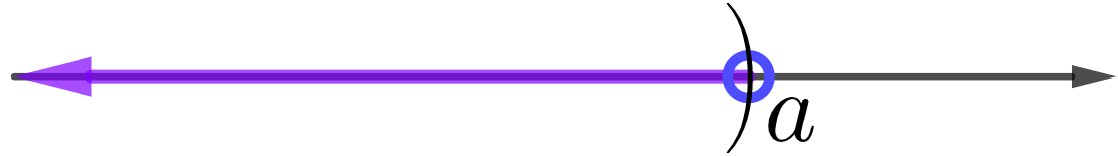
\includegraphics{figs/Interval-number-line-less-than.png} & 
\includegraphics{figs/Interval-number-line-greater-than.png} & 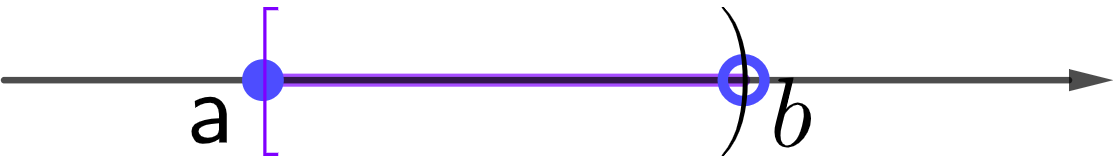
\includegraphics{figs/Interval-number-line-between.png} & 
\includegraphics{figs/Interval-number-line-beyond.png}\tabularnewline
\((-\infty, a)\) & \([b,\infty)\) & \([a, b)\) & \((-\infty, a]\cup (b,\infty)\)\tabularnewline
\bottomrule
\end{longtable}

\hypertarget{examples}{%
\section{Examples}\label{examples}}

\BeginKnitrBlock{rmdtip}
\textbf{Think backward.} To solve a problem, knowing what to expect helps you narrow down the gap step by step by comparing the goal and your achievement.

An inequality (equation) is solved if the unknown variable is isolated. That's what to be expected. To isolate the unknown variable, you use comparisons to determine what mathematical operations should be applied. When an operation is applied to one side, the same operation should also be applied to the other side. For inequalities, we also need to determine whether the inequality sign should be preserved or reversed according to the operation.
\EndKnitrBlock{rmdtip}

\BeginKnitrBlock{example}
\protect\hypertarget{exm:unnamed-chunk-6}{}{\label{exm:unnamed-chunk-6} }Solve the linear inequality
\[
2x+4>0.
\]
\EndKnitrBlock{example}

\BeginKnitrBlock{solution}
\iffalse{} {Solution. } \fi{}\[
\begin{aligned}
&  & 2x+4 & >0  \\
    \text{add $-4$}      &  & 2x   & >-4 \\
    \text{divide by $2$} &  & x    & >-2
\end{aligned}
\]
The solution set is \((-2, \infty)\).
\EndKnitrBlock{solution}

\BeginKnitrBlock{example}
\protect\hypertarget{exm:unnamed-chunk-8}{}{\label{exm:unnamed-chunk-8} }Solve the linear inequality
\[
-3x-4<2.
\]
\EndKnitrBlock{example}

\BeginKnitrBlock{solution}
\iffalse{} {Solution. } \fi{}\[
\begin{aligned}
                                        &  & -3x-4 & <2       \\
    \text{add $4$}                   &  & -3x   & <6  &  & \\
    \text{divide by $-3$ and switch} &  & x     & >-2
\end{aligned}
\]
The solution set is \((-2, +\infty)\).
\EndKnitrBlock{solution}

\BeginKnitrBlock{example}
\protect\hypertarget{exm:unnamed-chunk-10}{}{\label{exm:unnamed-chunk-10} }Solve the compound linear inequality
\[
x+2<3\quad \text{and}\quad -2x-3<1.
\]
\EndKnitrBlock{example}

\BeginKnitrBlock{solution}
\iffalse{} {Solution. } \fi{}\[
\begin{aligned}
    x+2 & <3 &  & \text{and} & -2x-3 & <1  \\
    x   & <1 &  &            & -2x   & <4  \\
    x   & <1 &  & \text{and} & x     & >-2
\end{aligned}
\]
That is \(-2<x<1\). The solution set is \((-2, 1)\).
\EndKnitrBlock{solution}

\BeginKnitrBlock{example}
\protect\hypertarget{exm:unnamed-chunk-12}{}{\label{exm:unnamed-chunk-12} }Solve the compound linear inequality\\
\[
-x+4>2 \quad \text{or} \quad 2x-5\geq -3.
\]
\EndKnitrBlock{example}

\BeginKnitrBlock{solution}
\iffalse{} {Solution. } \fi{}\[
\begin{aligned}
    -x+4 & >2  &  & \text{or} & 2x-5 & \geq -3 \\
    -x   & >-2 &  &           & 2x   & \geq 2  \\
    x    & <2  &  & \text{or} & x    & \geq 1
\end{aligned}
\]
That is \(x\geq 1\) or \(x< 2\). The solution set is \((-\infty, +\infty)\).
\EndKnitrBlock{solution}

\BeginKnitrBlock{example}
\protect\hypertarget{exm:unnamed-chunk-14}{}{\label{exm:unnamed-chunk-14} }Solve the compound linear inequality
\[
-4\leq\dfrac{2x-4}{3}<2.
\]
\EndKnitrBlock{example}

\BeginKnitrBlock{solution}
\iffalse{} {Solution. } \fi{}\[
\begin{array}{rcl}
    -4\leq  & \dfrac{2x-4}{3}    & <2  \\
    -12\leq & 2x-4         & <6  \\
    -8\leq  & 2x                & <10 \\
    -4\leq  & x               & <5  
\end{array}
\]
The solution set is \([-4, 5)\).
\EndKnitrBlock{solution}

\BeginKnitrBlock{example}
\protect\hypertarget{exm:unnamed-chunk-16}{}{\label{exm:unnamed-chunk-16} }Solve the compound linear inequality
\[
-1\leq \dfrac{-3x+4}{2}<3.
\]
\EndKnitrBlock{example}

\BeginKnitrBlock{solution}
\iffalse{} {Solution. } \fi{}\[
\begin{array}{rcl}
    -1\leq & \frac{-3x+4}{2}  & <3        \\
    -2\leq & -3x+4          & <6        \\
    -6\leq & -3x           & <2        \\
    2\geq  & x            & >-\frac23
\end{array}
\]
The solution set is \((-\frac23, 2]\).
\EndKnitrBlock{solution}

\BeginKnitrBlock{example}
\protect\hypertarget{exm:unnamed-chunk-18}{}{\label{exm:unnamed-chunk-18} }Suppose that \(-1\le x < 2\). Find the range of \(5-3x\). Write your answer in interval notation.
\EndKnitrBlock{example}

\BeginKnitrBlock{solution}
\iffalse{} {Solution. } \fi{}To get \(5-3x\) from \(x\), we need first multiply \(x\) be \(-3\) and then add \(5\).
\[
\begin{array}{rcl}
-1\leq & x          & < 2        \\
3\geq & -3x         & >-6        \\
8\geq & 5-3x      & >-1
\end{array}
\]
The range of \(5-3x\) is \((-1, 8]\).
\EndKnitrBlock{solution}

\BeginKnitrBlock{rmdtip}
\textbf{Understand the Problem.} Understanding the known, the unknown and the condition of the given problem is the key to solve the problem. Normally, by comparing the known and unknown, you will find the way to solve the problem.
\EndKnitrBlock{rmdtip}

\hypertarget{exercises}{%
\section{Exercises}\label{exercises}}

\BeginKnitrBlock{exercise}
\protect\hypertarget{exr:unnamed-chunk-21}{}{\label{exr:unnamed-chunk-21} }Solve the linear inequality. \textbf{Write your answer in interval notation.}

\begin{enumerate}
\def\labelenumi{\arabic{enumi}.}
\tightlist
\item
  \(3x + 7 \leq 1\)
\item
  \(2x-3>1\)
\end{enumerate}
\EndKnitrBlock{exercise}

\BeginKnitrBlock{exercise}
\protect\hypertarget{exr:unnamed-chunk-22}{}{\label{exr:unnamed-chunk-22} }Solve the linear inequality. \textbf{Write your answer in interval notation.}

\begin{enumerate}
\def\labelenumi{\arabic{enumi}.}
\tightlist
\item
  \(4x + 7 > 2x-3\)
\item
  \(3-2x \le x-6\)
\end{enumerate}
\EndKnitrBlock{exercise}

\BeginKnitrBlock{exercise}
\protect\hypertarget{exr:unnamed-chunk-23}{}{\label{exr:unnamed-chunk-23} }Solve the compound linear inequality. \textbf{Write your answer in interval notation.}

\begin{enumerate}
\def\labelenumi{\arabic{enumi}.}
\tightlist
\item
  \(3x+2>-1\) and \(2x-7\leq 1\)
\item
  \(4x -7< 5\) and \(5x-2\geq 3\)
\end{enumerate}
\EndKnitrBlock{exercise}

\BeginKnitrBlock{exercise}
\protect\hypertarget{exr:unnamed-chunk-24}{}{\label{exr:unnamed-chunk-24} }Solve the compound linear inequality. \textbf{Write your answer in interval notation.}

\begin{enumerate}
\def\labelenumi{\arabic{enumi}.}
\tightlist
\item
  \(-4\leq 3x+5<11\)
\item
  \(7\geq 2x-3\geq -7\)
\end{enumerate}
\EndKnitrBlock{exercise}

\BeginKnitrBlock{exercise}
\protect\hypertarget{exr:unnamed-chunk-25}{}{\label{exr:unnamed-chunk-25} }Solve the compound linear inequality. \textbf{Write your answer in interval notation.}

\begin{enumerate}
\def\labelenumi{\arabic{enumi}.}
\tightlist
\item
  \(3x-5>-2\) or \(10-2x\leq 4\)
\item
  \(2x + 7<5\) or \(3x-8\geq x-2\)
\end{enumerate}
\EndKnitrBlock{exercise}

\BeginKnitrBlock{exercise}
\protect\hypertarget{exr:unnamed-chunk-26}{}{\label{exr:unnamed-chunk-26} }Solve the compound linear inequality. \textbf{Write your answer in interval notation.}

\begin{enumerate}
\def\labelenumi{\arabic{enumi}.}
\tightlist
\item
  \(-2\leq \dfrac{2x-5}{3}<3\)
\item
  \(-1< \dfrac{3x+7}{2}\leq 4\)
\end{enumerate}
\EndKnitrBlock{exercise}

\BeginKnitrBlock{exercise}
\protect\hypertarget{exr:unnamed-chunk-27}{}{\label{exr:unnamed-chunk-27} }Solve the linear inequality. \textbf{Write your answer in interval notation.}
\[
\frac13x+1<\frac12(2x-3)-1
\]
\EndKnitrBlock{exercise}

\BeginKnitrBlock{exercise}
\protect\hypertarget{exr:unnamed-chunk-28}{}{\label{exr:unnamed-chunk-28} }Solve the compound linear inequality. \textbf{Write your answer in interval notation.}
\[
0\le \frac25-\frac{x+1}{3}< 1
\]
\EndKnitrBlock{exercise}

\BeginKnitrBlock{exercise}
\protect\hypertarget{exr:unnamed-chunk-29}{}{\label{exr:unnamed-chunk-29} }Suppose \(0< x \le 1\). Find the range of \(-2x+1\). \textbf{Write your answer in interval notation.}
\EndKnitrBlock{exercise}

\BeginKnitrBlock{exercise}
\protect\hypertarget{exr:unnamed-chunk-30}{}{\label{exr:unnamed-chunk-30} }Suppose that \(x+2y=1\) and \(1\leq x< 3\). Find the range of \(y\). \textbf{Write your answer in interval notation.}
\EndKnitrBlock{exercise}

\BeginKnitrBlock{exercise}
\protect\hypertarget{exr:unnamed-chunk-31}{}{\label{exr:unnamed-chunk-31} }A toy store has a promotion ``Buy one get the second one half price'' on a certain popular toy. The sale price of the toy is \$20 each. Suppose the store makes more profit when you buy two. What do you think the store's purchasing price of the toy is?
\EndKnitrBlock{exercise}
% 参考文献


% 插入 after_body.tex

\end{document}
